% ============================================================================
% 2026-09-29: the compounding exercise parked from Section 5.4
% (Section~\ref{sec:app_run_parked}: the paper's block-diagonal ridge under the
% session-bar recalibration), re-run for the HEADLINE forecast under the
% 16:00-bar recalibration of Table~\ref{tab:close_option_rules}.  Every number
% below is a macro from generated/appendix_close_compounding.tex, written by
% experiments/close_compounding_headline.py from results/close_compounding/*.csv;
% nothing is typed by hand.  The two recalibrations are never set side by side.
% Input from main.tex after sections/appendix_close_murphy_splits, so this
% continues Appendix D.
% ============================================================================
% AUTO-GENERATED by experiments/close_compounding_headline.py from results/close_compounding/*.csv -- do not edit.
\begingroup\footnotesize\setlength{\tabcolsep}{3pt}
\begin{longtable}{llrrrrr}
\caption{Compounding at a fixed $f=0.03$ of wealth per day under the 16:00-bar recalibration, 866 days: terminal wealth $W_T=\prod_t(1+f\,q_tR_t)$, annualized log-growth $g$, the largest fall of wealth from its running peak, the worst single-day wealth factor $1+f\min_t R'_t$, and the ruin bound $1/|\min_t R'_t|$ (the sample's worst day). The headline, the paper's block-diagonal ridge scored the same way, and always short, at both fills.}\label{tab:app_compounding_headline}\\
\toprule
series & fill & $W_T$ & $g$ & max DD & worst day & ruin bound \\
\midrule
\endfirsthead
\caption[]{(continued)}\\
\toprule
series & fill & $W_T$ & $g$ & max DD & worst day & ruin bound \\
\midrule
\endhead
\bottomrule
\endlastfoot
headline sign(s) & mid & 20.18 & +0.87 & 34\,\% & 0.837 & 0.18 \\
headline sign(s) & crossed & 8.55 & +0.62 & 38\,\% & 0.832 & 0.18 \\
reference sign(s) (this scorer) & mid & 3.89 & +0.40 & 42\,\% & 0.837 & 0.18 \\
reference sign(s) (this scorer) & crossed & 1.62 & +0.14 & 50\,\% & 0.832 & 0.18 \\
always short & mid & 0.86 & -0.04 & 55\,\% & 0.691 & 0.10 \\
always short & crossed & 0.33 & -0.32 & 74\,\% & 0.671 & 0.09 \\
\end{longtable}
\endgroup

\newcommand{\cmpF}{0.03}
\newcommand{\cmpHW}{20.2}
\newcommand{\cmpHG}{+0.87}
\newcommand{\cmpHDD}{34}
\newcommand{\cmpHWorst}{16}
\newcommand{\cmpHRuin}{0.18}
\newcommand{\cmpHWX}{8.5}
\newcommand{\cmpHGX}{+0.62}
\newcommand{\cmpHDDX}{38}
\newcommand{\cmpRW}{3.9}
\newcommand{\cmpRG}{+0.40}
\newcommand{\cmpRWX}{1.6}
\newcommand{\cmpAW}{0.86}
\newcommand{\cmpAG}{-0.04}
\newcommand{\cmpARuin}{0.10}
\newcommand{\cmpAWX}{0.33}
\newcommand{\cmpNAll}{220}
\newcommand{\cmpNPosMid}{218}
\newcommand{\cmpNPosX}{208}
\newcommand{\cmpWLoMid}{0.6}
\newcommand{\cmpWHiMid}{20.4}
\newcommand{\cmpWLoX}{0.2}
\newcommand{\cmpWHiX}{8.6}
\newcommand{\cmpHRankMid}{2}
\newcommand{\cmpHRankX}{2}
\newcommand{\cmpNYears}{5}
\newcommand{\cmpNPosYears}{4}
\newcommand{\cmpNegYears}{2022 is $-0.01$}
\newcommand{\cmpNPosYearsX}{4}
\newcommand{\cmpNegYearsX}{2022 is $-0.19$}
\newcommand{\cmpYearsMid}{2020: $+0.87$, 2021: $+0.79$, 2022: $-0.01$, 2023: $+1.29$, 2024: $+2.15$}
\newcommand{\cmpYearsX}{2020: $+0.44$, 2021: $+0.48$, 2022: $-0.19$, 2023: $+1.11$, 2024: $+1.96$}

\subsection{The Headline Forecast Compounded at a Fixed Fraction of Wealth}
\label{sec:app_compounding_headline}

\paragraph{What is computed.} The fixed-fraction exercise of
Section~\ref{sec:close_option_methods} --- a share $f=\cmpF$ of current wealth deployed
as straddle premium every day, the same on every day and for every rule, wealth
$W_T=\prod_t(1+f\,q_tR_t)$, the annualized mean of $\log(1+fR'_t)$ as the growth rate,
every wealth factor asserted positive --- repeated for the headline's $\mathrm{sign}(s)$
positions under the 16:00-bar recalibration, on the 866 days and at both fills, beside the
paper's block-diagonal ridge scored the same way and always short
(Table~\ref{tab:app_compounding_headline}, Figure~\ref{fig:app_compounding_headline}).
The midpoint frame is the one Section~\ref{sec:app_run_parked} reports for the paper's
forecast under the other recalibration; the crossed frame pays the ask and hits the bid on
every day.

\paragraph{Reading.} At the midpoint the headline turns one unit of wealth into \cmpHW{}
over the sample (annualized log-growth \cmpHG{}), with a maximum wealth drawdown of
\cmpHDD{} percent and a worst single day that removes \cmpHWorst{} percent of wealth; the
ruin bound $1/|\min_t R'_t|$ is \cmpHRuin{} for the headline and \cmpARuin{} for always
short, so \cmpF{} sits inside both. Across the spread it ends at \cmpHWX{}
(log-growth \cmpHGX{}, drawdown \cmpHDDX{} percent). The paper's forecast scored the same
way ends at \cmpRW{} at the midpoint (\cmpRG{}) and \cmpRWX{} across the spread; always
short ends at \cmpAW{} (\cmpAG{}) and \cmpAWX{}. Of the \cmpNAll{} distinct forecasts of the
master table (the rest-of-day check rows, exact copies of their per-bar twins, left out),
\cmpNPosMid{} compound above one unit at the midpoint (terminal wealth \cmpWLoMid{}
to \cmpWHiMid{}; the headline ranks \cmpHRankMid{}) and \cmpNPosX{} across the spread
(\cmpWLoX{} to \cmpWHiX{}; the headline ranks \cmpHRankX{}). By calendar year, annualized
from the days traded in each, the headline's midpoint log-growth is positive in
\cmpNPosYears{} of \cmpNYears{} years (\cmpYearsMid{}) and across the spread in
\cmpNPosYearsX{} (\cmpYearsX{}).

\begin{figure}[H]
\centering
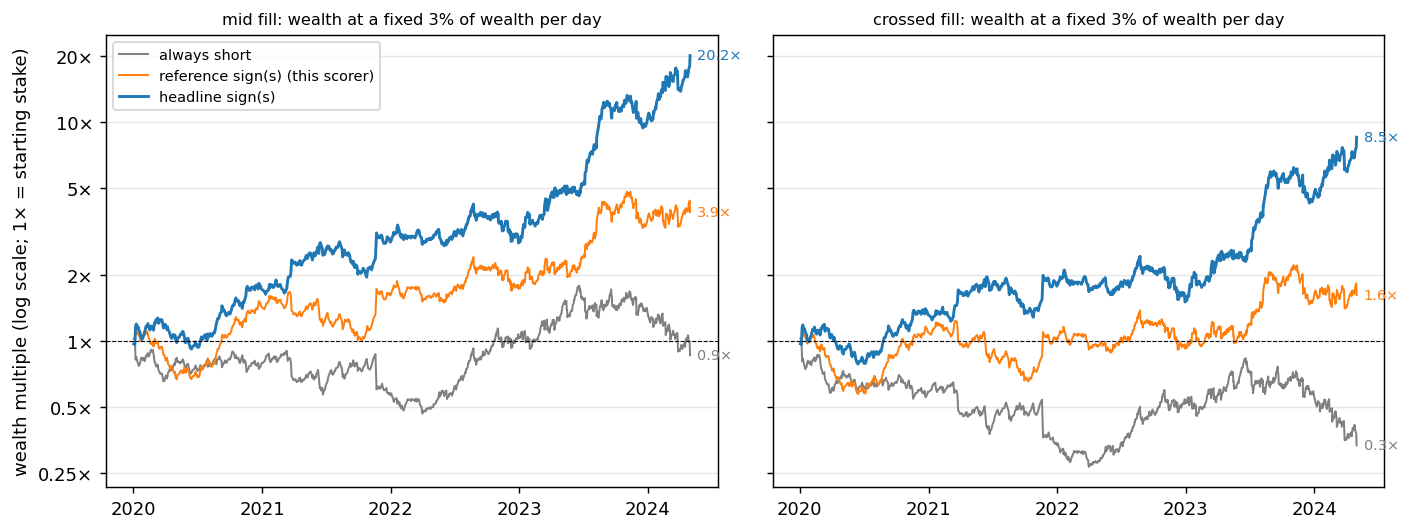
\includegraphics[width=\textwidth]{../results/close_compounding/wealth_headline.png}
\caption{Wealth at a fixed \cmpF{} of wealth per day, 866 days, under the 16:00-bar
recalibration: the headline's $\mathrm{sign}(s)$, the paper's block-diagonal ridge scored the
same way, and always short; midpoint fill (left) and crossed spread (right), log scale
(source: \texttt{results/close\_compounding/fixedfrac\_headline.csv}).}
\label{fig:app_compounding_headline}
\end{figure}
